Die Sweepline sweept von links nach rechts, also entlang er $x$-Achse.

\begin{description}
\item[site] ist ein Punkt in der Ebene.
\item[beach line] teilt die Ebene in zwei Bereiche. Oberhalb der beach line sind alle Bereiche die potentiell zu den Voronoi Regionen der jeweiligen Punkte gehören werden. Unterhalb der beach line alle Punkte zu denen noch keine Aussage getroffen werden kann. Die Punkte auf der beach line sind equidistant zum zugehörigen Punkt und zur sweep line.
\item[spikes] zukünftige Voronoi Kanten. An Schnittpunkten von Spikes entstehen zukünftige Voronoi Knoten.
\item[breakpoint] sind die Schnittpunkte der Parabeln, dort befinden sich auch die Spikes, also durch die zwei Schnittpunkte verläuft genau ein Spike.
\item[site Event] tritt auf, wenn die Sweepline einen Punkt ("`site"') trifft.
\item[circle Event] tritt auf, wenn Kreisbögen verschwinden. D.h. ein circle event entsteht aus einem site event. Wenn sich zwei Spikes schneien, der Kreis durch die zugehörigen Punkte und dann ganz unten auf dem Kreis ist eine neues circle event.
\item[sweep line status (SLS)] enthält die Topologie der Beachline in Form einer Liste, sozusagen die Kreisbögen und die dazugehörigen Punkte und eine Information darüber, durch welches Event ein Kreisbogen verschwindet.
\item[event point schedule (EPS)] enthält site events und circle events. Die Priorität ist durch die $x$-Koordinate gegeben, d.h. tritt das Event weiter links auf, so ist die Priorität höher. Initialisiert wird die priority queue mit allen zu Beginn gegebenen Punkten.
\end{description}

\paragraph*{Initialisierung}
\begin{description}
\item[EPS] $(0,0)[\text{se1}]$, $(1,2)[\text{se2}]$, $(2,3)[\text{se3}]$, $(4,3)[\text{se4}]$
\item[beachline] $\emptyset$
\end{description}

\newpage

\paragraph*{EVENT 1 - site event $(0,0)$}
\begin{description}
\item[EPS] $(1,2)[\text{se2}]$, $(2,3)[\text{se3}]$, $(4,3)[\text{se4}]$
\item[beachline] $a_1 \rightarrow (0,0)$
\end{description}

\begin{figure}[h]
\begin{center}
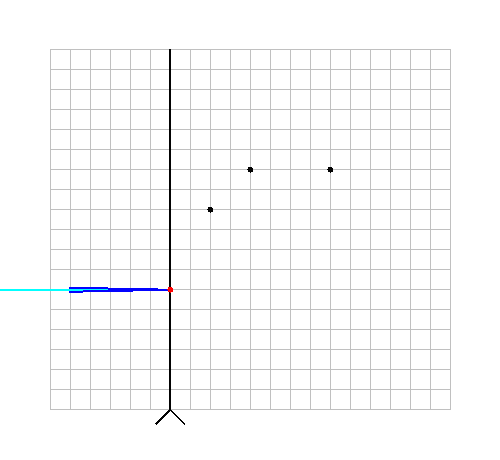
\includegraphics[width=7cm]{capture1}
\end{center}
\caption{Schritt 1}
\label{fig:c1}
\end{figure}

Kein circle event und keine neuen Kanten.

\newpage

\paragraph*{EVENT 2 - site event $(1,2)$}
\begin{description}
\item[EPS] $(2,3)[\text{se3}]$, $(4,3)[\text{se4}]$
\item[beachline]
$a_{1.1} \rightarrow (0,0)$,\\
$a_2 \rightarrow (1,2)$,\\
$a_{1.2} \rightarrow (0,0)$\\
\end{description}

\begin{figure}[h]
\begin{center}
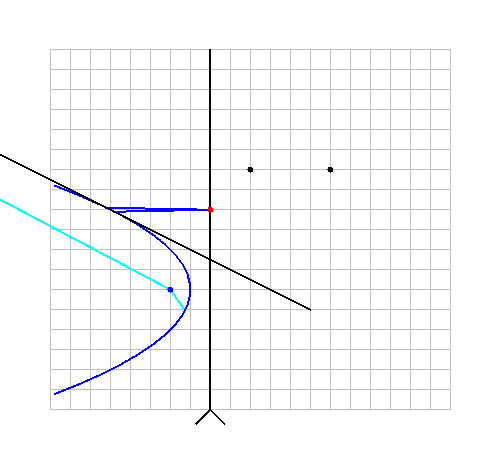
\includegraphics[width=7cm]{capture2}
\end{center}
\caption{Schritt 2}
\label{fig:c2}
\end{figure}

Kein circle event, eine neue Kante, die $(0,0)$ von $(1,2)$ trennt.

\newpage

\paragraph*{EVENT 3 - site event $(2,3)$}
\begin{description}
\item[EPS] $(4,3)[\text{se4}], (11 + \sqrt{130}, -3)[\text{ce1}]$
\item[beachline]
$a_{1.1} \rightarrow (0,0)$\\
$a_{2.1} \rightarrow (1,2)$\\
$a_3 \rightarrow (2,3)$\\
$a_{2.2} \rightarrow (1,2)[\text{delete at ce1}]$\\
$a_{1.2} \rightarrow (0,0)$
\end{description}

\begin{figure}[h]
\begin{center}
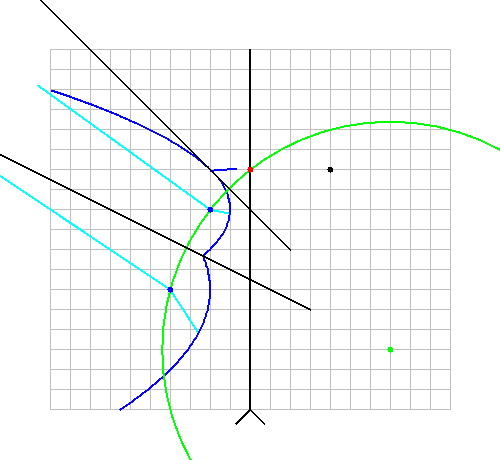
\includegraphics[width=7cm]{capture3}
\end{center}
\caption{Schritt 3}
\label{fig:c3}
\end{figure}

Der Schnittpunkt $(11, -3)$ der beiden Spikes ist ein evtl. zukünftiger Voronoi Knoten. Der Fußpunkt des grünen Kreises wird als neues circle event $(11 + \sqrt{130}, -3)[ce1]$ für $a_{2.2}$ der EPS hinzugefügt.

Für $a_{2.1}$ ensteht kein valides circle event, da der Kreis keine ''Rechtsdrehung'' beschreibt.

\newpage

\paragraph*{EVENT 4 - site event $(4,3)$}
\begin{description}
\item[EPS] $(6 + \sqrt{20}, 2)[\text{ce2}], (11 + \sqrt{130}, -3)[\text{ce1}]$
\item[beachline]
$a_{1.1} \rightarrow (0,0)$\\
$a_{2.1} \rightarrow (1,2)$\\
$a_{3.1} \rightarrow (2,3)$\\
$a_4 \rightarrow (4,3)$\\
$a_{3.2} \rightarrow (2,3)[\text{delete at ce2}]$\\
$a_{2.2} \rightarrow (1,2)[\text{delete at ce1}]$\\
$a_{1.2} \rightarrow (0,0)$
\end{description}

Der Schnittpunkt der beiden letzen Spikes $(6,2)$ ist ein evtl. zukünftiger Voronoi Knoten. Der Fußpunkt dieses Kreises wird als neues circle event  $(6 + \sqrt{20}, 2)[\text{ce2}]$ der EPS hinzugefügt und rutscht in der priority queue ganz nach vorne.

Für $a_{3.1}$ ensteht kein valides circle event.

\begin{figure}[h]
\begin{center}
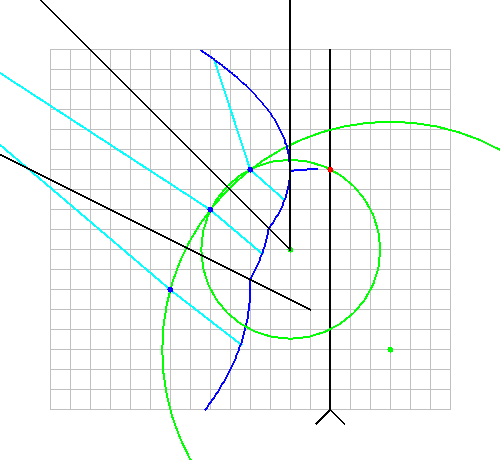
\includegraphics[width=7cm]{capture4}
\end{center}
\caption{Schritt 4}
\label{fig:c4}
\end{figure}

\newpage

\paragraph*{EVENT 5 - circle event $(6 + \sqrt{20}, 2)$}
\begin{description}
\item[EPS] $(11 + \sqrt{130}, -3)[\text{ce3}]$
\item[beachline]
$a_{1.1} \rightarrow (0,0)$\\
$a_{2.1} \rightarrow (1,2)$\\
$a_{3} \rightarrow (2,3)$\\
$a_4 \rightarrow (4,3)$\\
$a_{2.2} \rightarrow (1,2)[\text{delete at ce3}]$\\
$a_{1.2} \rightarrow (0,0)$
\end{description}

\begin{figure}[h]
\begin{center}
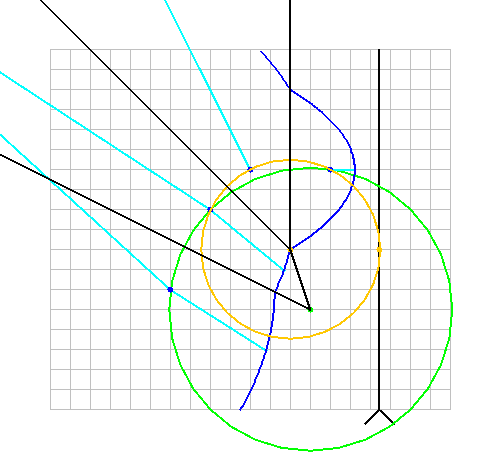
\includegraphics[width=7cm]{capture5}
\end{center}
\caption{Schritt 5}
\label{fig:c5}
\end{figure}

Ein Parabelbogen verschwindet, der Voronoi Knoten bei $(6,2)$ ist nun fest. Für $a_{2.2}$ wird ein neues circle event mit Mittelpunkt $(7,-1)$ bei $(7 + \sqrt{50}, -1)[\text{ce3}]$ erzeugt, das $ce1$ obsolet macht.

\newpage

\paragraph*{EVENT 6 - circle event $(7 + \sqrt{50}, -1)$}
\begin{description}
\item[EPS] $\emptyset$
\item[beachline]
$a_{1.1} \rightarrow (0,0)$\\
$a_{2} \rightarrow (1,2)$\\
$a_{3} \rightarrow (2,3)$\\
$a_4 \rightarrow (4,3)$\\
$a_{1.2} \rightarrow (0,0)$
\end{description}

\begin{figure}[h]
\begin{center}
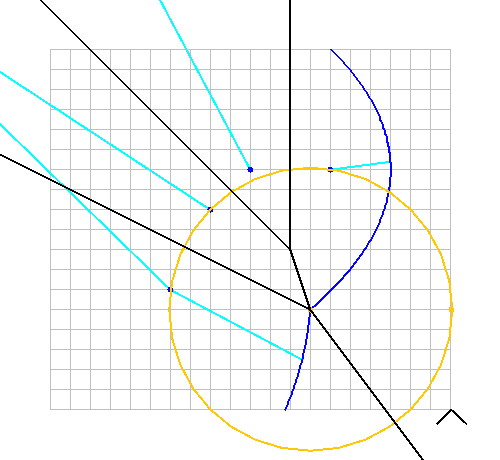
\includegraphics[width=7cm]{capture6}
\end{center}
\caption{Schritt 6}
\label{fig:c6}
\end{figure}

Ein Parabelbogen verschwindet, der Voronoi Knoten bei $(7,-1)$ ist nun fest.

\newpage

\begin{figure}[h]
\begin{center}
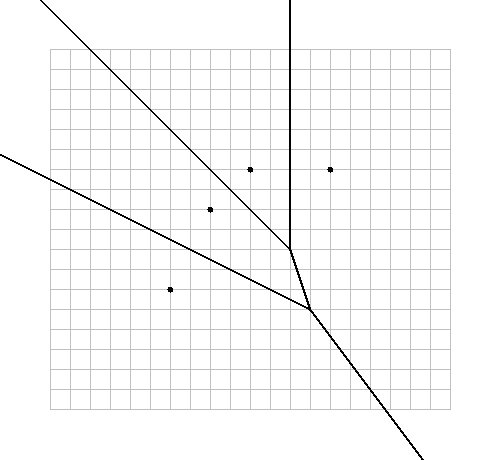
\includegraphics[width=7cm]{capture7}
\end{center}
\caption{Schritt 7}
\label{fig:c7}
\end{figure}

Abschließend wird geprüft, ob mit den Parabelsegmenten in der beachline noch ungebundene Kanten verknüpft sind, die sich zwischen den Segmenten schneiden. Dies ist hier nicht der Fall, womit das Voronoi-Diagramm feststeht.

Btw: die Bilder sind aus unserer \emph{Implementierung} ;)